\section{Introduction to Graph Databases}

Nowadays a huge number of different databases systems exist. You always must select the best suiting one for your specific use case. Data is often ordered in relations between objects, like different cities and their connecting streets. 
If there is the possibility to structure your data in the database the same way as the data is structured in real life, you may get a speed and usability advantage out of that. The best solution to picture these structures is to use the graph. That is why graph databases have been developed, which now will be presented to you.

\subsection{Graph Databases}

Graph databases use graph structure to order data in the database. There is more than one solution for using graphs. The main aspects of the first are nodes and edges, which are essential for the database structure \cite[pp. 1-4]{RobinsonWebberEifrem.2013}.
The connection between the nodes are the relations of the data. In the example picture below \cite[para. 1]{Rouse.2016}, you can see how graph databases work with the nodes and their relations. For example you can see the married couple Julie and Bob.

\begin{figure}[H]
	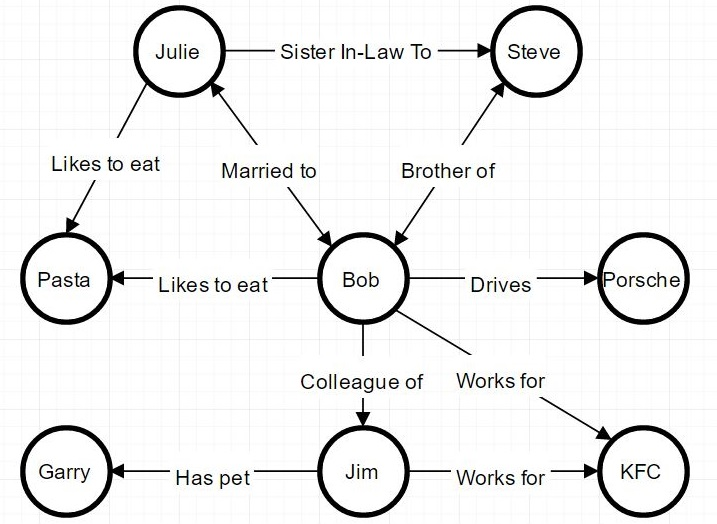
\includegraphics[width=\linewidth,keepaspectratio]{images/neo4j/IntroExampleGraph.JPG}
	\caption{ExampleGraph}
\end{figure}

You can also build property graphs, which you can use for routing. For example, you can find the shortest way from one city to another. The special thing about property graphs is, that attributes can be added to the nodes and edges. So you can store further information in your graph \cite[p.3]{RodriguezNeubauer.2010}.

The second one is used for the semantic web and concentrates on triples. Semantic web stands for machine processable web. In the semantic web the W3C consortium defined a framework how to work with the triples \cite["Overview", para. 1]{W3C.2014}. It is called Resource Description Framework and its structure is like following:

\begin{itemize}
	\item First part: subject, where the relation starts.
	\item The second: predicate, the relation
	\item The third: object, where the predicate points to.
\end{itemize}  

Despite you can see the same node and edge structure, it is different to the property graphs. In Resource Description Framework, which is the most common used framework, you can only build connections between the nodes, but you can neither set properties to the nodes nor to the edges.

\subsection{Neo4j}

Neo4j - developed by Neo Technology - is one of the first and up to now the most popular graph database implementation. Neo4j is more than five times popular than the second graph database - OrientDB  \cite[para. 1]{SolidITGmbH.2017}.\\
Its first Version was released in 2010 after three years of development. It is called as transactional, disk based database, which follows the ACID principle \cite["Neo4j Internals", para. 4]{NeoTechnologyInc.2017b}. The implementation is in Java and can be used in two different license models. The Community and the Enterprise Edition.\\
The Community Edition is free, but only running on a single node. You can use all the features of Neo4j without high availability through clustering and hot backup. 
These additional modules are coming with the Enterprise Edition only. There are some further categorizations for the Enterprise version like the test licenses Evaluation, the Educational and the Neo4j Loves Open Source licenses \cite["About Neo4j Licenses", para. 1]{NeoTechnologyInc.2017a}.\\
Neo4j uses Cypher as query language. With indexing and the labels of the graph it helps to accelerate the queries, which is one of the main advantage of using graph databases and especially Neo4j.

Now you get a deeper insight into Neo4j and its data structure.

\section{Data Structures}

In opposite to the bulk of NoSQL databases Neo4j as a graph database is focused on the relationships between data.
Therefore the data structure is based on two components: nodes and relationships. Both of them can contain a variety of informations.
Let's start with the nodes. Each node consists of a JSON object which defines its properties, so the nodes can be compared to documents in MongoDB for example. In the definition of this node properties you can use anything, that's provided by the JSON standard. In a library for example we could have books with properties about their title, page number or publication date.
With this properties we get the ability to store data and in connection with the later introduced cypher query language we can search for nodes by them. But currently searches would be executed over the whole graph and any node can contain different properties.
\cite["Nodes", para. 3]{NeoTechnologyInc.2017c} \cite[p. 80]{Gupta.2015} \cite[slide 20-21]{Hunger.2013}

\begin{figure}[H]
	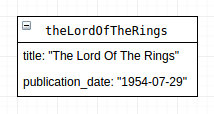
\includegraphics[width=\linewidth,keepaspectratio]{images/neo4j/data-structure/single-node.png}
	\caption{Single Book Node}
\end{figure}

To structure the data, every node can be labeled. This labels can be interpreted as  a typing. Looking back at our library example we could create nodes labeled as “book”, “author” or “borrower”. By labeling the node we organize them in sets, like the MongoDB collections or SQL tables.
Beside the better structure we achieve a more efficient searching, because the amount of data to search in can be reduced right at the beginning, by the definition of the node set (label) to search in.
At this point we have nodes with properties organized in sets by their labels, but no relationships.
\cite["Labels", para. 2]{NeoTechnologyInc.2017c} \cite[slide 26-27]{Hunger.2013}

\begin{figure}[H]
	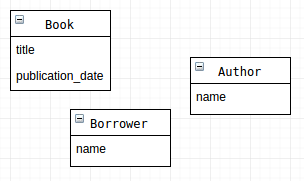
\includegraphics[width=\linewidth,keepaspectratio]{images/neo4j/data-structure/labeled-nodes.png}
	\caption{Labeled Node Sets}
\end{figure}

The relationships in Neo4j are quite similar to the nodes. They are also able to take properties in form of JSON objects and has labels to define their type or in this case better to say their function. In the library example a relationship between book and borrower could be labeled as “borrowed” and contains properties like “borrowDate”, “returnDate” or maybe “rating”. Here we should also have a look at a good structure, so it would be better to extract the rating and put it in another relationship like “read”.
The main and obvious difference are the two connected nodes. So every relationship needs exactly two nodes connected to it. But they do not have to be different, so it'’'s possible to point a relationship on its own origin. Naturally the node labels are irrelevant here, so relationships can be defined inside and between node sets.
\cite["Relationships", para. 1]{NeoTechnology2017c.2017c} \cite[p. 81-82]{Gupta.2015} \cite[slide 22-25]{Hunger.2013}

\begin{figure}[H]
	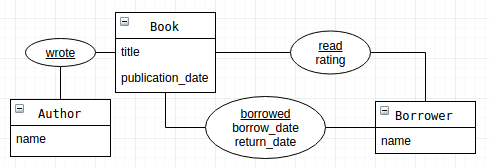
\includegraphics[width=\linewidth,keepaspectratio]{images/neo4j/data-structure/node-relationships.png}
	\caption{Related Nodes}
\end{figure}

After looking at the elements of the Neo4j data structure, we will now have a look at how we create this structure in our database instance.
At first it'’'s necessary to create some nodes. Therefore we use the CREATE command followed by round brackets to define the node itself. The first element of the node definition is an optional variable name at first to save the reference to the created node, if needed. After this a colon and label name is required to define the node set. The label doesn'’'t need to be defined before using it here. At last we enter the JSON object with our node properties and close the definition brackets.
\cite["Create a Record for Yourself", para. 1]{NeoTechnologyInc.2017d} \cite[p. 80]{Gupta.2015}

\begin{lstlisting}[frame=single, caption=Create Database, label=creategraphdb]
CREATE ( variable:LABEL {} )
CREATE ( theLordOfTheRings:Book { title: 'The Lord Of The Rings', publication_date: '1954-07-29' } )
CREATE ( jrrTolkien:Author { name: 'J. R. R. Tolkien' } )
CREATE ( johnSmith:Borrower { name: 'John Smith' } )
\end{lstlisting}

Secondly we can create the relationships. Thanks to the ascii-art syntax it'’'s easy to understand the create statements. It starts again with a CREATE and is followed by round brackets. In this case this brackets can contain a node definition again, but also a simple variable name to reference an existing node. After the brackets a hyphen connects the first node to the relationship definition part surrounded by square brackets. This definition is structured like the node definition: optional variable name, label, JSON object. An ascii arrow (“->”) connects the closing square bracket with the second node, this relation will point to. In the style of the first node we have here round brackets with a variable or a  whole node definition.
\cite["Create a Record for Yourself", para. 1]{NeoTechnologyInc.2017d} \cite[p. 81-82]{Gupta.2015}

\begin{lstlisting}[frame=single, caption=Create Relationships, label=creategraphrelationships]
CREATE (sourceNode)-[ variable:LABEL {} ]->(targetNode)
CREATE (jrrTolkien)-[ :WROTE ]->(theLordOfTheRings)
CREATE (johnSmith)-[ :BORROWED { borrowDate: '2017-03-15', returnDate: '2017-04-14' } ]->(theLordOfTheRings)
\end{lstlisting}

Below you can have a look at the created graph of the simple example.

\begin{figure}[H]
	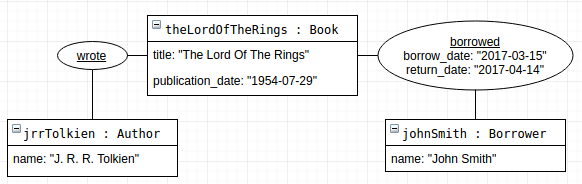
\includegraphics[width=\linewidth,keepaspectratio]{images/neo4j/data-structure/sample-graph.png}
	\caption{Sample Graph}
\end{figure}

\section{Cypher Language}

Cypher is Neo4j's open graph query language. It was newly created to match the data-structures of Neo4j and to fulfill the special needs of Graph-Databases.
In addition it's based on SQL to allow an easy entry point for developers, which already had to work with SQL. \cite["About Cypher", para. 1]{NeoTechnologyInc.2017d}
Cypher's syntax provides a familiar way to match patterns of nodes and relationships in the graph.
Cypher is also a relatively simple but still very powerful language.
Very complicated database queries can easily be expressed through Cypher.
This allows users to focus on their domain instead of getting lost in database access because it allows the user to state what he wants to select, insert, update or delete from his graph data without requiring him to describe exactly how to do it.

\paragraph{Example}

Cypher contains a variety of clauses. 
Among the most common are: MATCH and WHERE. \cite["A few words about Cypher", para. 3]{NeoTechnologyInc.2017f}
These functions are slightly different than in SQL.
MATCH is used for describing the structure of the pattern searched for, primarily based on relationships.
WHERE is used to add additional constraints to patterns.
For example, the below query will return all movies starting with "T", and return its cast as a collection:
\begin{lstlisting}[frame=single, caption=Cypher Example, label=cypherexample]
MATCH (actor:Person)-[:ACTED_IN]->(movie:Movie)  
WHERE movie.title STARTS WITH "T"  
RETURN movie.title AS title, collect(actor.name) AS cast  
ORDER BY title ASC LIMIT 10;
\end{lstlisting}

\paragraph{ASCII-Art and Nodes}

Cypher uses ASCII-Art to represent patterns. It surrounds nodes with parentheses which look like circles, e.g. \textbf{(node)}. \cite["Nodes", para. 1]{NeoTechnologyInc.2017d}

\begin{figure}[H]
	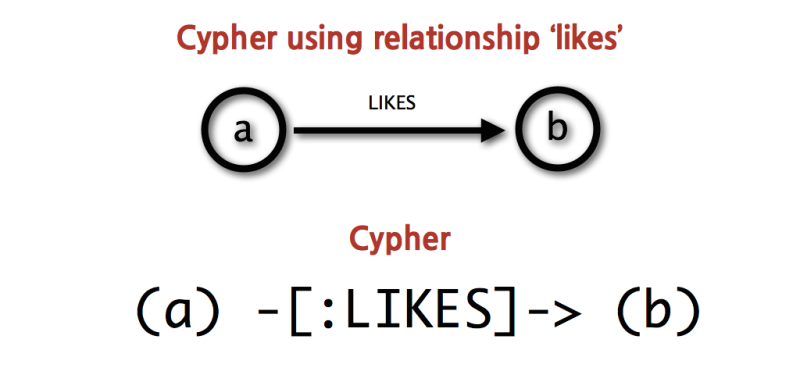
\includegraphics[width=\linewidth,keepaspectratio]{images/neo4j/cypher_pattern_simple.png}
	\caption{node ascii art}
\end{figure}

To reference a node at a later time, it can be stored in a variable like (p) for person or (t) for thing.
In real-world queries, there would probably be longer, more expressive variable names like (person) or (thing).
If the node is not relevant to the question, the parenthesis can also be empty ().

\paragraph{Relationships}

To fully utilize the power of graph databases complex patterns between the nodes can be expressed.
Relationships are basically an arrow \textbf{-->} between two nodes. \cite["Relationships", para. 1]{NeoTechnologyInc.2017d}
Additional information can be placed in square brackets inside of the arrow.

This can be

\begin{itemize}
	\item relationship-types like \textbf{-[:KNOWS|:LIKE]->}
	\item a variable name \textbf{-[rel:KNOWS]->} before the colon
	\item additional properties \textbf{-[{since:2010}]->}
	\item structural information for paths of variable length \textbf{-[:KNOWS\\*..4]->}
\end{itemize} 
\cite{NeoTechnologyInc.2017d} ("Relationships", para. 3)

\begin{lstlisting}[frame=single, caption=Create a Record, label=gcar]
CREATE (you:Person {name:"You"})
RETURN you
\end{lstlisting}
\textbf{CREATE} creates nodes with labels and properties.

\begin{figure}[H]
	
\includegraphics[width=\linewidth,keepaspectratio]{images/neo4j/you.png}
	\caption{graph you}
\end{figure}

\begin{lstlisting}[frame=single, caption=Create Relations, label=gcrl]
MATCH (you:Person {name:"You"})
FOREACH (name in ["Tobias","Kai","Manuel"] |
CREATE (you)-[:FRIEND]->(:Person {name:name}))
\end{lstlisting}
\textbf{FOREACH} allows the execution of update operations for each element of a list.

\begin{lstlisting}[frame=single, caption=Show Relations, label=gshrl]
MATCH (you {name:"You"})-[:FRIEND]->(yourFriends)
RETURN you, yourFriends
\end{lstlisting}

\begin{figure}[H]
	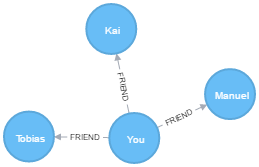
\includegraphics[width=\linewidth,keepaspectratio]{images/neo4j/friends.png}
	\caption{graph friends}
\end{figure}

\section{Comparison with other Database Systems}

The following chapters will compare graph databases, especially Neo4j with other database systems such as relational databases and NoSQL (not only SQL) databases. In addition to plain comparisons there will also be some examples how graph databases can be used with other systems to maximmize the advantages of each system.

\subsection{Comparison with Relational Databases}

This chapter will give a basic overview of the similiarities and differences between graph databases and relational databases. More specifically this chapter will focus on Neo4j and SQL. 
In Neo4j relationships are first-class citizens. In SQL these relationships can only be created by using foreign keys and therefore Neo4j eliminates foreign keys. Each node contains a list of relationship-records. These relationship-records are organized by type and direction and can hold additional attributes. When you would normally run a JOIN-operation these records are used. This is the biggest advantage graph databases have over relational databases: The costs of expensive search and match operations are eliminated.
This leads to much higher performance levels than those of relational databases.
In addition the data models of graph databases are simpler and more expressive as seen in the below images \cite[pp. 9-10]{HungerBoydLyon.2016}.

\begin{figure}[H]
	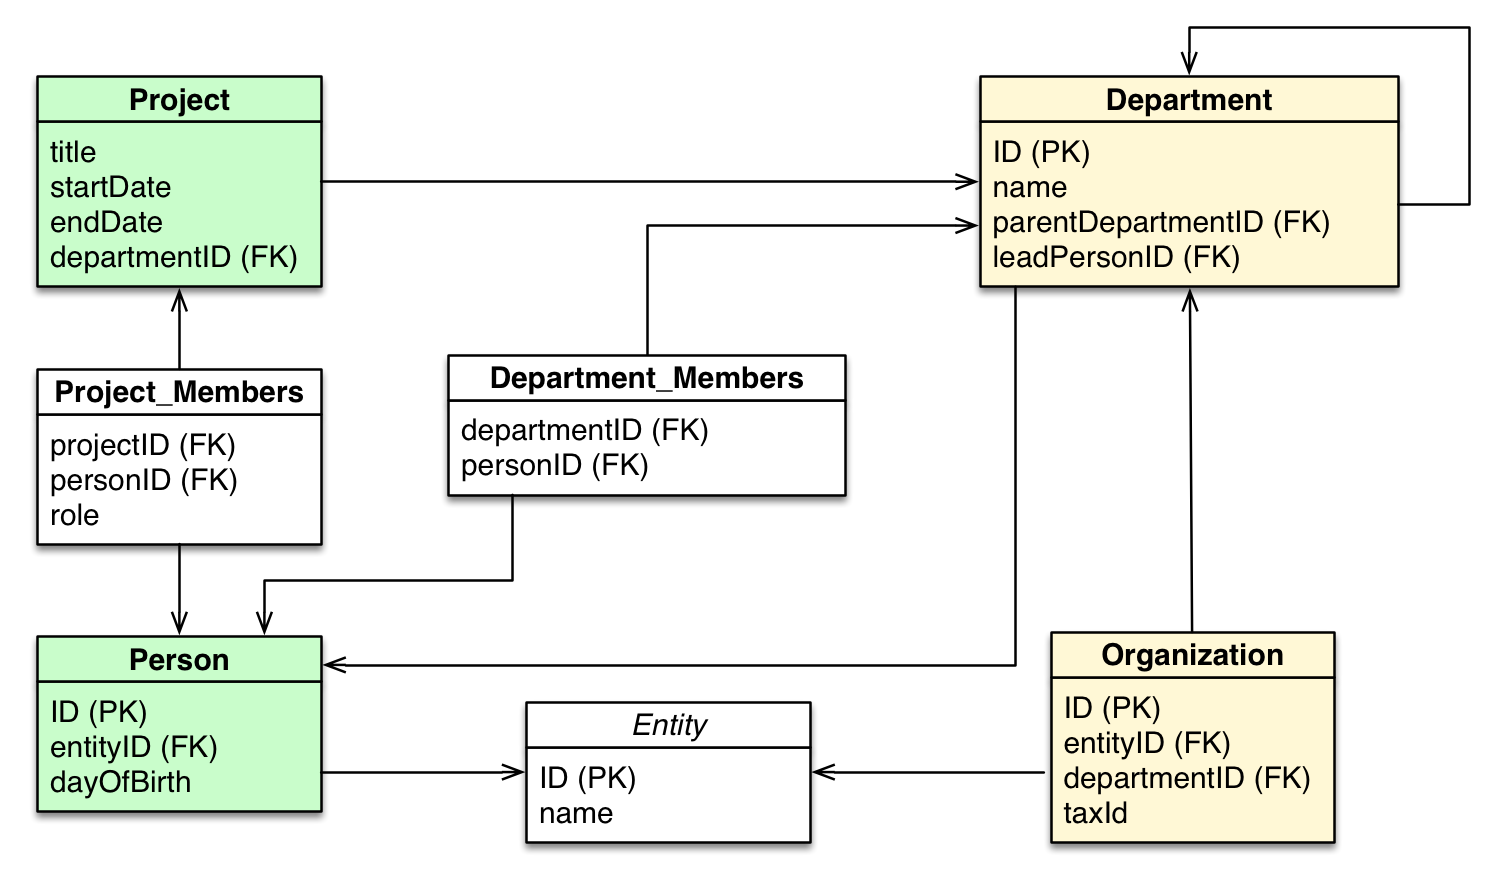
\includegraphics[width=\linewidth,keepaspectratio]{images/neo4j/organization_relational.png}
	\caption{SQL data model}
\end{figure}

\begin{figure}[H]
	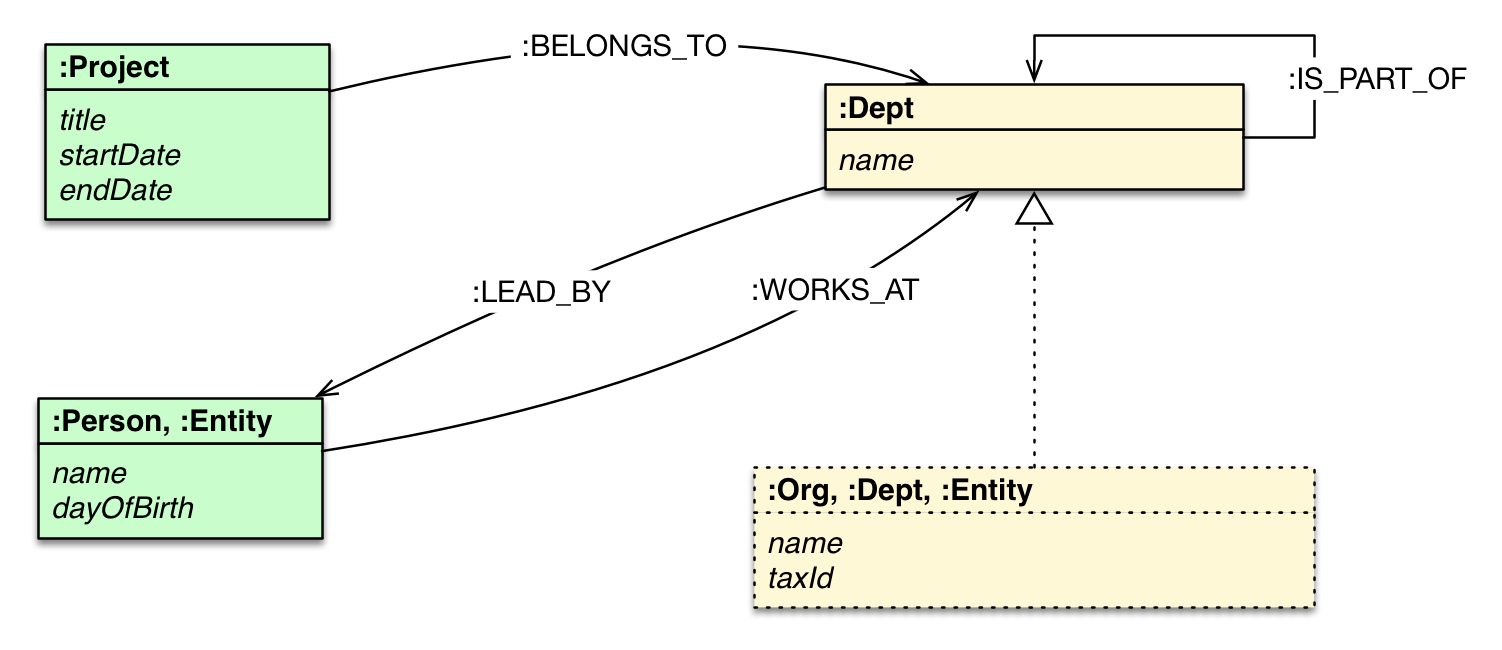
\includegraphics[width=\linewidth,keepaspectratio]{images/neo4j/organization_graph.png}
	\caption{Neo4j data model}
\end{figure}

Like SQL Neo4j also supports the transactional concepts (ACID). That means that data is never lost after it has been commited to the database.
The query language is pretty similiar, but cypher, the query language of Neo4j, is more expressive.
Following is a short comparison of the same transaction in SQL and Cypher. This example also demonstrates the strength of Cypher by eliminating two JOIN-operations.

\begin{lstlisting}[frame=single, caption=Cypher Statement, label=gcystm]
MATCH (p:Person)<-[:EMPLOYEE]-(d:Department)
WHERE d.name = "IT Department"
RETURN p.name
\end{lstlisting}

\begin{lstlisting}[frame=single, caption=SQL Statement, label=gsqlstm]
SELECT name FROM Person
LEFT JOIN Person_Department
ON Person.Id = Person_Department.PersonId
LEFT JOIN Department
ON Department.Id = Person_Department.DepartmentId
WHERE Department.name = "IT Department"
\end{lstlisting}

\subsection{Comparison with NoSQL Databases}

Since relationships are very important in graph databases, it's quite difficult to compare them with NoSQL databases, since they lack relations. Following statement by Webber and Robinson (2015) explains this scenario in a good way:
\begin{quotation}
	Most NoSQL databases store sets of disconnected aggregates. This makes it difficult to use them for connected data and graphs.
	One well-known strategy for adding relationships to such stores is to embed an aggregate'’'s identifier inside the field belonging to another aggregate — effectively introducing foreign keys.
	But this requires joining aggregates at the application level, which quickly becomes prohibitively expensive.
\end{quotation} \cite[p. 15]{Webber.Robinson.2015}.

\subsection{Integration with other Database Systems}
This section will describe how to use Neo4j together with other database systems in a very basic way. It will not go in-depth and there will be no code examples to keep it as simple as possible.
To get the advantages of each database system, data needs to be stored in each database with its own data models. This is called polyglot programming: using multiple different languages, here multiple different database systems. There are existing tools for different database systems which can be used as some kind of connector to another system. The connectors let the other system subscribe to update events, so the data can be inserted in one database system and then added in the other system. The developers of MongoDB for example have created a tool called "mongo-connector" where other applications can listen for update events. This enables a one-way synchronization with Neo4j. Of course all the data model transformations have to be made manually, but once set up the full potential of both databases can be used.

\section{Conclusion}

In the end you can say that Graph databases, and therefore also Neo4j, don't need joins to achieve relationships, since they are already first-class citizens. This has a huge impact on performance, since join-operations are very expensive.
As Neo4j holds its data as JSON it has a similiar structure to document based databases and could be used together. That way you can get the advantages of both systems. The only disadvantage is the need to store the whole data twice, which requires more storage.

In general Neo4j fullfills the CAP-theorem in points of \textbf{c}onsistency and \textbf{a}vailablity and doesn't provide \textbf{p}artition tolerance. Because Neo4j is relationship-oriented, trying to achieve partition tolerance can cause many side effects and complex queries would decrease the performance considerable.

Neo4j has many use cases. For example it is used by companies such as Walmart for real-time recommendations, Ebay for logistics, LinkedIn as a representation for their Social Network and TomTom for geo-routing. An interessting fact at this point was published by the Neo4j staff. They said Neo4j is not used by Facebook, which "they should" change \cite[para. 5]{Neo4jStaff.2011}.

Neo4j is mainly used for relational analytics and is hence not efficient unless you have many joins. The following chart will enforce this statement.

\begin{figure}[H]
	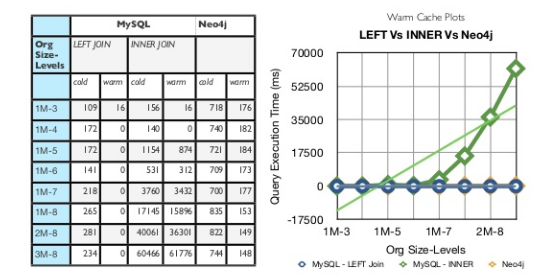
\includegraphics[width=\linewidth,keepaspectratio]{images/neo4j/neo4j_joins.png}
	\caption{neo4j sql comparison}
\end{figure}  
\cite[slide 19]{Dalal.2014}.

As shown in the graph, Neo4j's full potential unleashes when many join-operations are executed as the query execution time stays constantly low, whereas the execution time for inner joins in MySQL rises exponentially. Another performance aspect is, that Neo4j in its second version can automatically index often used Nodes and gets an additional speed advantage at run time.

Overall Neo4j is quite unique, but has high potential in the sector of relational databases.
It is useful to perform complex relational data queries and can be used for many different business cases.
It is still the most popular graph database and some weaknesses can be handled by using Neo4j with another NoSQL database together.